\chapter{Betrag}

Autor: Marc Mittner

\section{Der absolute Betrag}

\subsection{Definition}

Für eine reele Zahl x ist der Betrag definiert als: 

\Large
$ | x | =  \left\{ ^{ \ \  x \ , \ x \geq 0}_{-x \ , \ x < 0} \right. $
\normalsize

\subsection{Die Betragfunktion}
Graph der Betragfunktion $ f(x) \ = \ |x| $:
\begin{center}
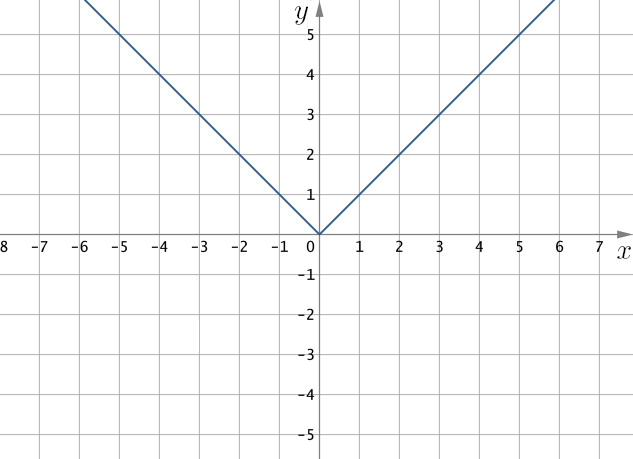
\includegraphics[width=0.5\textwidth]{img/Betragsfkt.png}
\end{center}
Betragfunktion:
\begin{itemize}
\item symmetrisch zur y-Achse 
\item $y \geq \ 0$ für alle Werte $ x \in \mathbb{R} $.
\end{itemize}

%\pagebreak
\subsection{Beispiele}
Gleichungen mit Beträgen werden durch Fallunterscheidung gelöst.
\begin{enumerate}
 \item $ | x-1 | \ = \ 3 $

Fallunterscheidung

1.Fall:
\[ (x \ - \ 1) \ = \ 3 \] 
\[ x \ = \ 4 \] 

%\newpage

2. Fall:
\[-(x \ - \ 1) \ = \ 3 \]
\[ x \ = \ -2 \]


\item $ (x \ + \ 3)^2 \ = \ 4 $
\[ \rightarrow | x+3 | \ = \ 2 \]
Fallunterscheidung

1. Fall:
\[ +(x \ + \ 3) \ = \ 2 \]

2. Fall:
\[ -(x \ + \ 3) \ = \ -2 \]
\end{enumerate}
